%%%%%%%%%%%%%%%%%%%%%%%%%%%%%%%%%%%%%%%%%%%%%%%%%%%%%%%%%%%%%%%%%%%%
% Overivew
%%%%%%%%%%%%%%%%%%%%%%%%%%%%%%%%%%%%%%%%%%%%%%%%%%%%%%%%%%%%%%%%%%%%

\section{Model Interlocking Assemblies}
\label{sec:model}
%
%In this section, we introduce our conceptual representation of interlocking assemblies using a family of directed graphs. We show how this graph-based representation leads to an efficient algorithm to {\em test} interlocking. 
%In Section~\ref{sec:approach} we then explain how to effectively employ this representation and algorithm to {\em design} interlocking assemblies.
%%\TODO{one more assumption: we focus on (dis)assemblies parts with translational motions, e.g., do not consider taking a part by rotating it first and then doing the translation.}


\begin{figure}[!t]
	\centering
	%\vspace*{-3.5mm}
	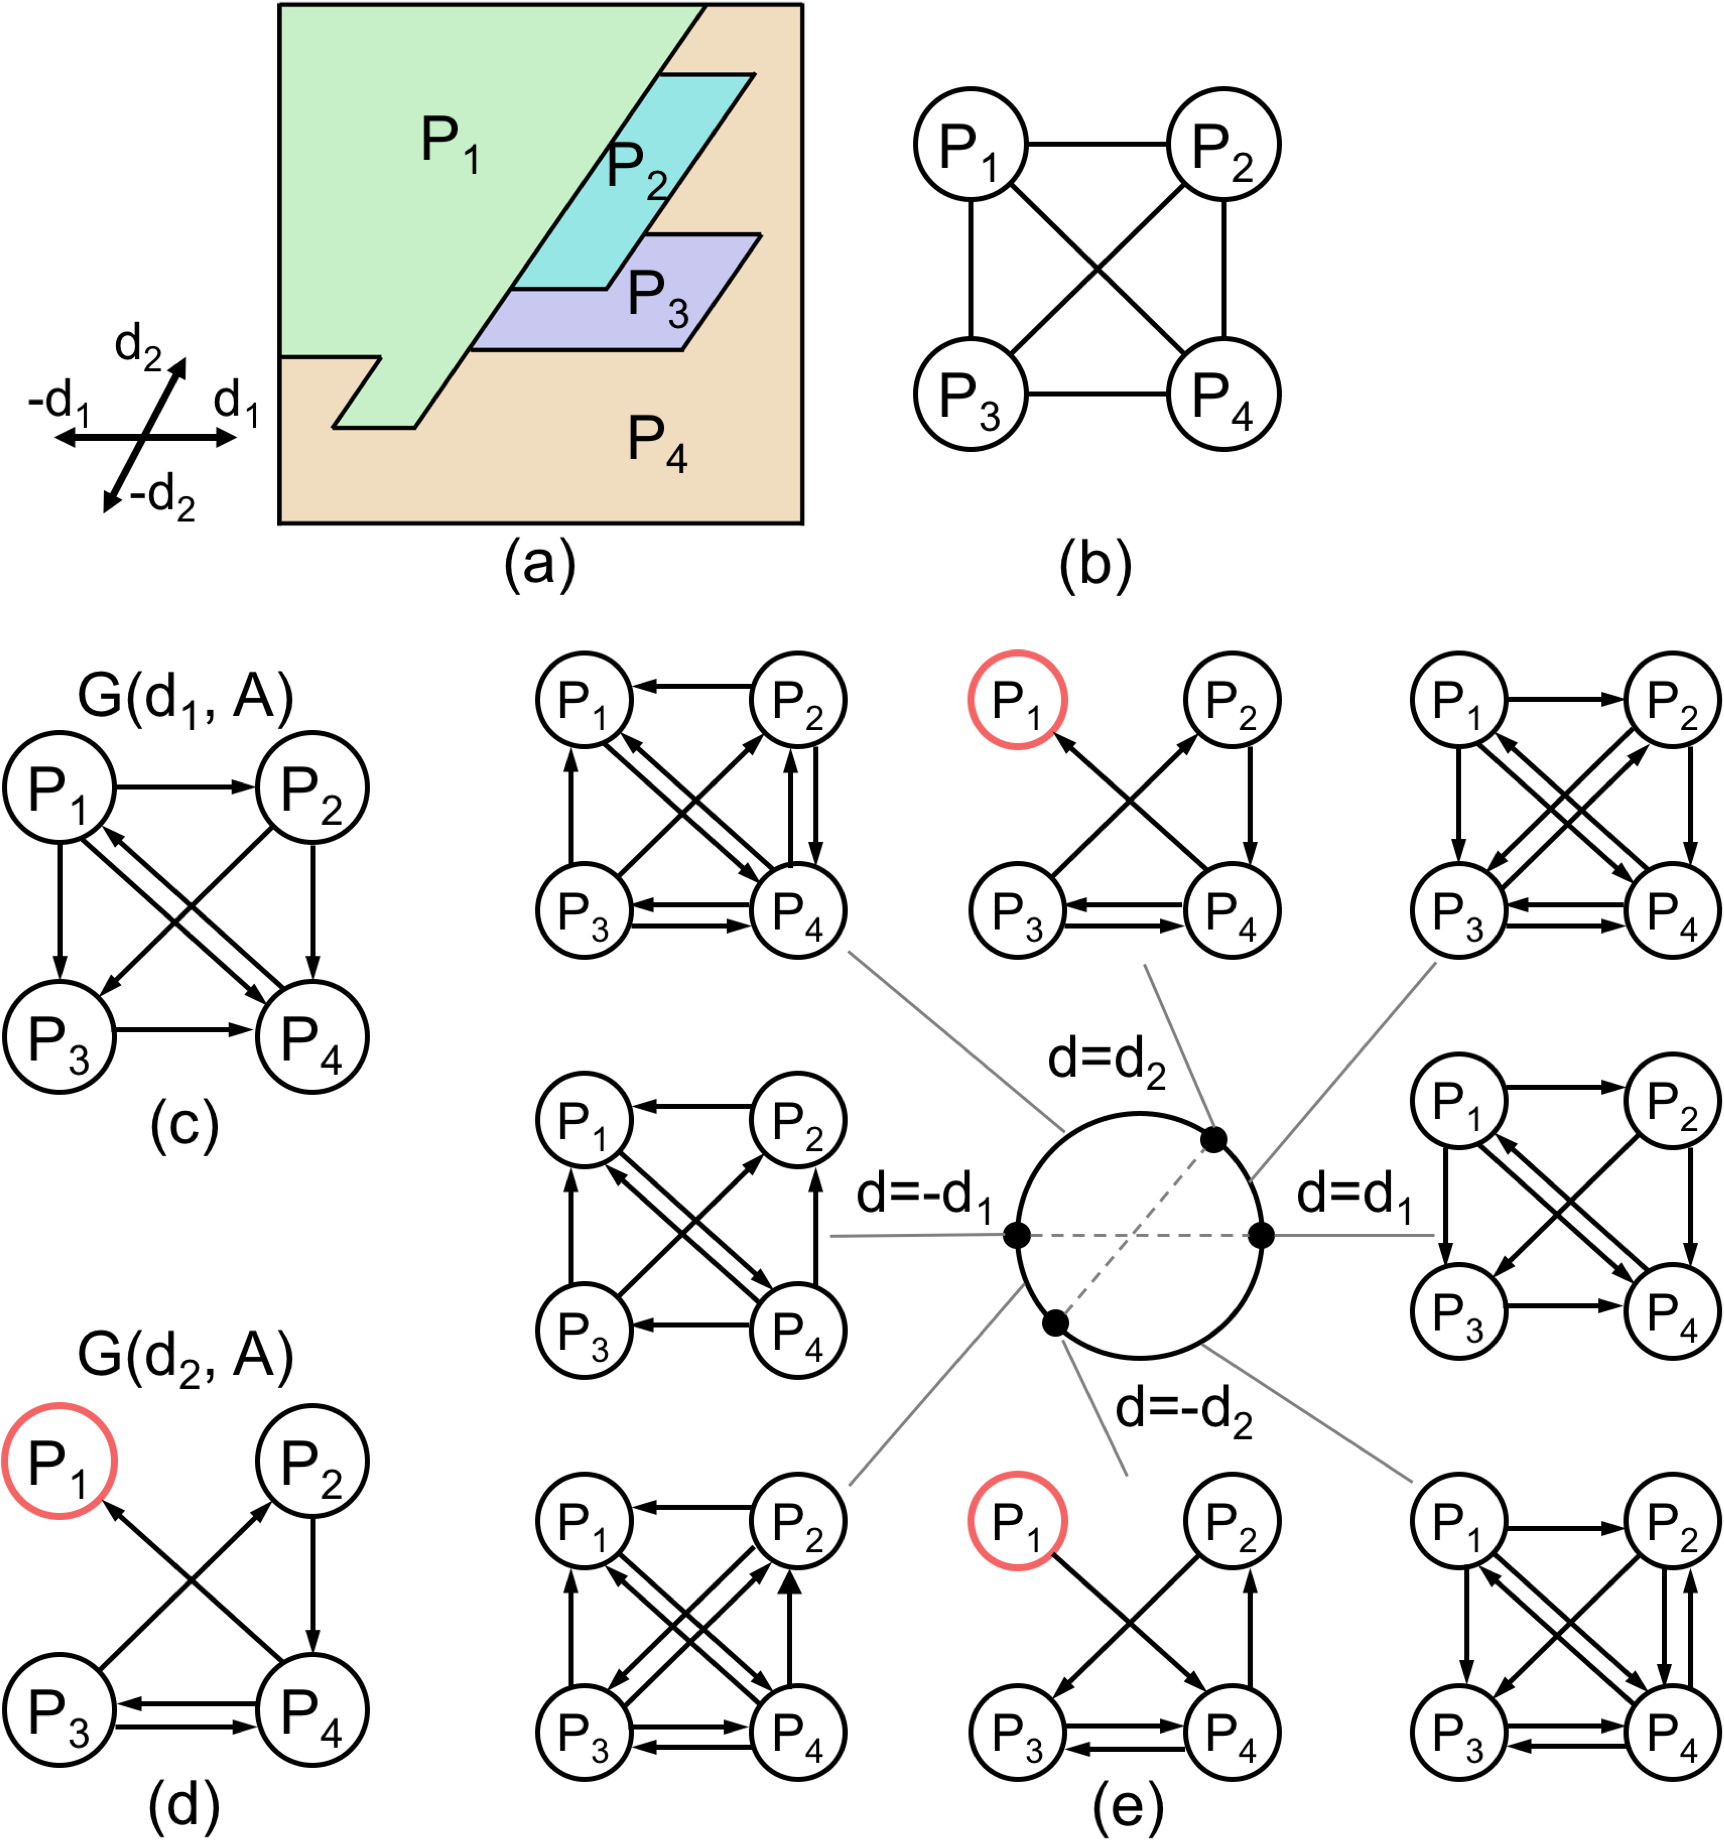
\includegraphics[width=8.00cm]{images/NDBG.png}
	\vspace*{-2.5mm}
	\caption{Example DBGs and NDBG.
		(a\&b) A 2D interlocking assembly and its parts-graph, where the key $P_1$ is movable along $d_2$;
		(c\&d) Two DBGs of the assembly; and
		(e) NDBG of the assembly.
		A part with zero out-degree or in-degree in a DBG is highlighted with a red circle. 
		%\Mark{I would still consider using crossing edges, I think it will make it easier to read.I would also expand the figure  to reach to full width, i.e. add more space.}
	}
	\vspace*{-4.0mm}
	\label{fig:NDBG}
\end{figure}

\subsection{Graph Model}
\label{subsec: graphmodel}

%%%%%%%%%%%%%%%%%%%%%%%%%%%%%%%%%%%%%%%%%%%%%%%%
% Our Inputs
%%%%%%%%%%%%%%%%%%%%%%%%%%%%%%%%%%%%%%%%%%%%%%%%

Consider an assembly $\mathbf{A}$, made of $n$ parts $P_1$, $...$, $P_n$.
We make the following assumptions:
1) each part $P_i$ is rigid; 
2) neighboring parts have planar surface contact only; and 
%(e.g., corner-surface and edge-surface contacts are not considered); and
3) $\mathbf{A}$ can be disassembled by single-part translational motions, i.e., part rotation is not required and all other parts remain fixed when removing a part.


%%%%%%%%%%%%%%%%%%%%%%%%%%%%%%%%%%%%%%%%%%%%%%%%
% Base DBGs
%%%%%%%%%%%%%%%%%%%%%%%%%%%%%%%%%%%%%%%%%%%%%%%%

\vspace*{1.0mm}
\noindent
{\bf Directional Blocking Graph (DBG).}\  
We denote as $G(d, A)$ the {\em directional blocking graph} of assembly $\mathbf{A}$ for translation along direction $d$. 
This directed graph has nodes representing the parts of $\mathbf{A}$ and directed edges $e_{i \rightarrow j}$ from $P_i$ to $P_j$  if and only if $P_j$ prevents any translational motion of $P_i$ along $d$. 
In other words, $e_{i \rightarrow j}$ can be read as ``$P_i$  is blocked by $P_j$" in direction $d$. 
See Figure~\ref{fig:NDBG}(c\&d) for two examples.

If $G(d, A)$ is {\em strongly connected}, i.e. if every node can be reached from every other node, no part or part group is movable along $d$; see Figure~\ref{fig:NDBG}(c). 
A part group $\mathbf{S}$ of $\mathbf{A}$ is locally free to translate in direction $d$ ($-d$), if and only if the out-degree (in-degree) of $\mathbf{S}$ in $G(d, A)$ is zero; see $P_1$ in Figure~\ref{fig:NDBG}(d).
%there is no edge in $G(d, A)$ connecting parts in $\mathbf{S}$ to parts in $\mathbf{A} \setminus \mathbf{S}$; see $P_1$ in Figure~\ref{fig:NDBG}(d) for an example.
%since there is no out-edge connecting it with the other nodes in the graph; see Figure~\ref{fig:NDBG}(d). 


\vspace*{1.0mm}
\noindent
{\bf Non-directional Blocking Graph (NDBG).} \
We represent the set of all translation directions in 2D by the unit circle denoted as $C$.
For every pair of parts in contact in $\mathbf{A}$, we draw the diameter that is parallel with the contact line.
The drawn diameters partition $C$ into an arrangement of regions, for which the corresponding DBG $G(d, A)$ remains constant when $d$ varies over a region.
For any pair of parts in 
\vspace*{5mm}
\setlength{\columnsep}{13pt}
\begin{wrapfigure}{r}{0.32\columnwidth}
	\vspace{-6pt}
	\centering
	\hspace{-4pt}
	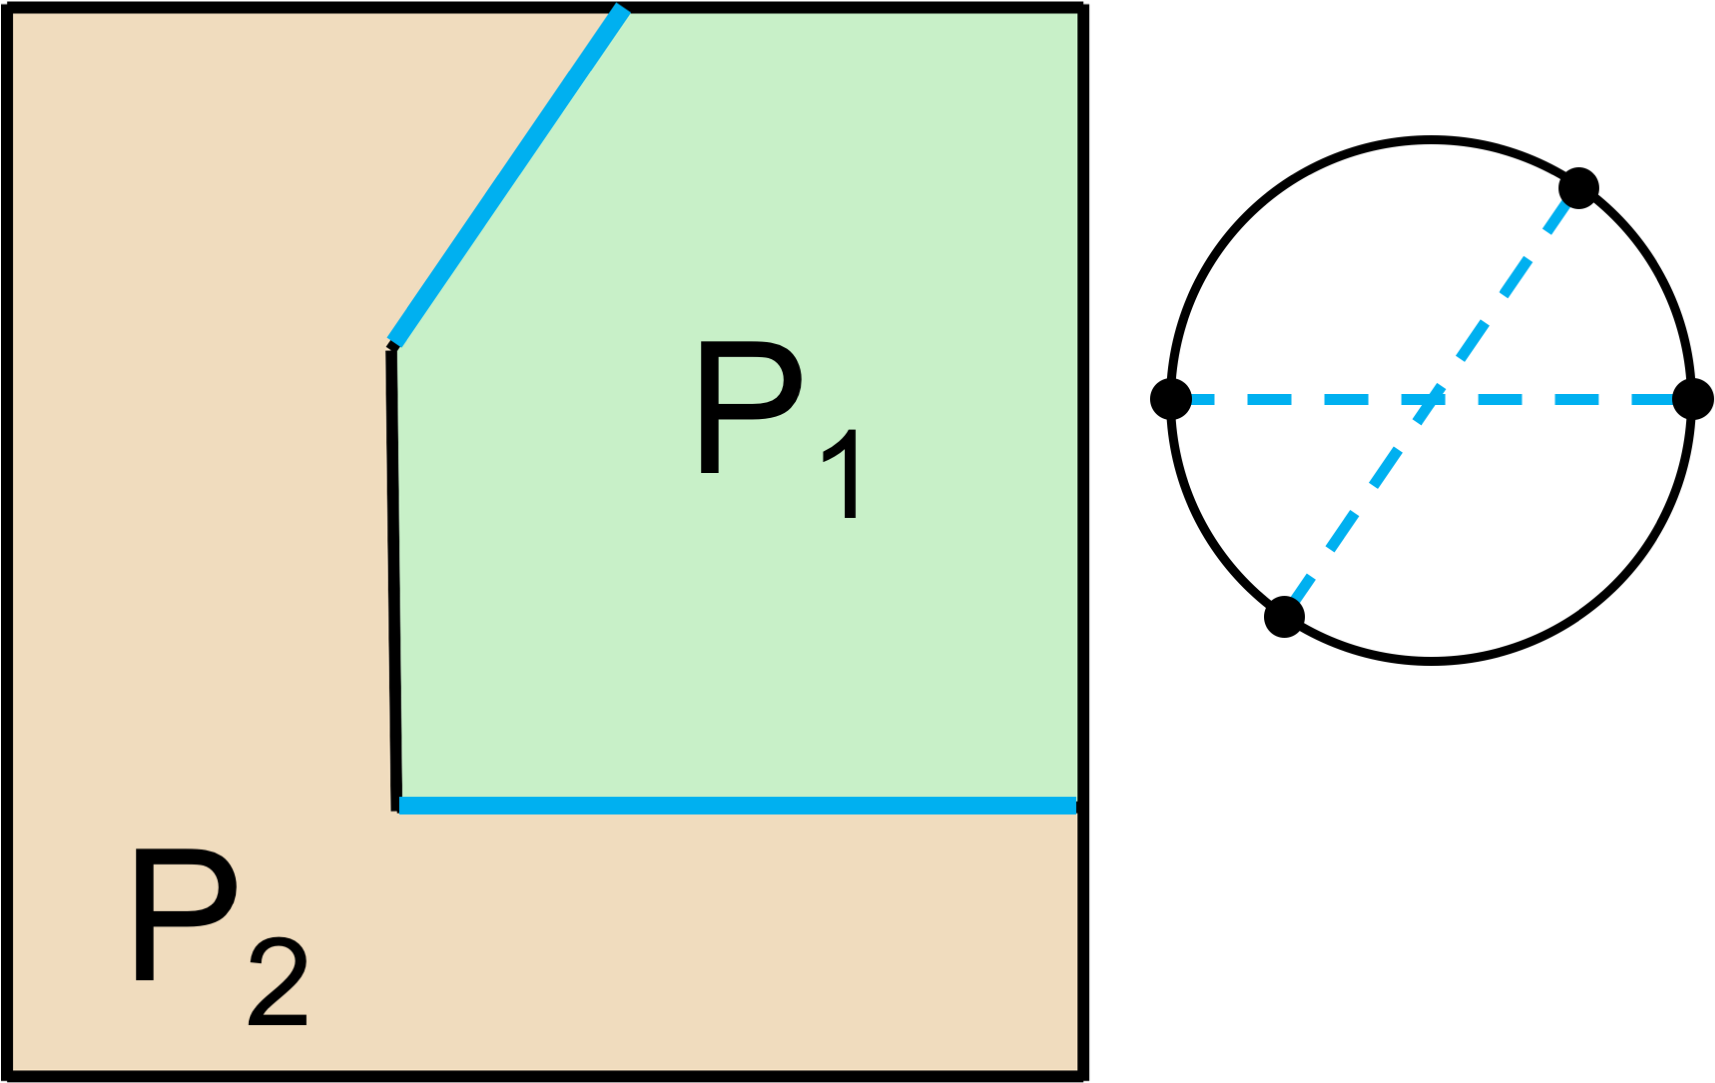
\includegraphics[width=0.32\columnwidth]{images/NDBG_Diameter.png}
	\vspace{-5pt}
\end{wrapfigure}
contact (e.g., $P_1$ and $P_2$ in the inset), if there are more than two contact lines, we only retain the two diameters of $C$ (e.g., two contact lines in blue) which bound the cone of directions in which one part is free to translate relative to the other.
The arrangement of points and intervals on $C$ and the associated DBGs form the {\em non-directional blocking graph} of $\mathbf{A}$; see Figure~\ref{fig:NDBG}(e).
% which represents the blocking relations among parts in $\mathbf{A}$ for all possible translation directions.
The NDBG for a 3D assembly can be built similarly by constructing DBGs for each regular region of a unit sphere that represents all possible translation direction in 3D; please refer to~\cite{Wilson-1994-GeometricReasoning} for more details.

\vspace*{1.0mm}
\noindent
{\bf Base Directional Blocking Graphs.} \
An NDBG represents the parts blocking relations with redundancy in two aspects.
First, the DBG corresponding to an arc in $C$ can be derived by performing union operations on the DBGs associated with the two end points of the arc; see again Figure~\ref{fig:NDBG}(e).
%This is because the blocking relations for $d = d_1$ and $d = d_2$ are the extreme case
%by performing union of the edges in these two graphs since \TODO{give a reason here}.
Second, we can obtain $G(-d, A)$ from $G(d, A)$ easily by reversing the direction of every edge in $G(d, A)$ due to the reciprocity of  blocking relations among the parts.

Therefore, it is sufficient to model the blocking relations in $\mathbf{A}$ by using only a set of {\em base DBGs} denoted as $\{G(d, A)\}$, which we select as the DBGs corresponding to the end points in a half circle of $C$.
For example, two DBGs in Figure~\ref{fig:NDBG}(c\&d) form $\{G(d, A)\}$.
We call the set of directions corresponding to the base DBGs as {\em base directions}, denoted as $\{d\}$.
%The number of base DBGs (as well as base directions) is $O(n^2)$ since every pair of parts provides either two (in contact) or zero (no contact) diameters in $C$.
The number of base DBGs (as well as base directions) is $O(n^2)$ since every pair of parts provides at most two diameters in $C$.  
%\Mark{Does this mean two contact parts cannot be blocked only along a single direction?}
%\Peng{You are right. Two contact parts are possible to provide one diameter. Text has been revised accordingly.}
%\Mark{better to have a figure showing 3D base DBGs}

%Hence, if a part of part group is movable along the direction within the arc, it must be movable also along the direction corresponding to one of the end points.
%Hence, when identifying movable parts or part groups,  we only need to test each direction corresponding to the end points (e.g., $-x, +x, -y, +y$ in Figure~\ref{fig:NDBG}).



%%%%%%%%%%%%%%%%%%%%%%%%%%%%%%%%%%%%%%%%%%%%%%%%
% Test Interlocking 
%%%%%%%%%%%%%%%%%%%%%%%%%%%%%%%%%%%%%%%%%%%%%%%%

\subsection{Testing Interlocking}
\label{subsec: testinginterlocking}
In an interlocking assembly, every part and every part group are immobilized for all possible translation directions, except a single key.
To test immobilization of a part group $\mathbf{S}$, we need to compute blocking relations between $\mathbf{S}$ and $\mathbf{A}-\mathbf{S}$:  the part group $\mathbf{S}$ is immobilized if $\mathbf{S}$ is blocked by $\mathbf{A}-\mathbf{S}$ in all translation directions.
Explicitly testing interlocking by checking immobilization of every part and every part group has exponential time complexity. 
However, treating each part group $\mathbf{S}$ independently ignores significant redundancies in the blocking relations across the parts.
%This huge complexity mainly arises from the redundancy of recomputing blocking relations for every parts group $\mathbf{S}$ by considering it as a totally new unit.
% rather than utilizing the computed blocking relations of $\mathbf{S}$'s component parts.
%
We exploit these redundancies and propose a more efficient approach to test global interlocking. 
The key idea is to utilize the blocking relations encoded in the set of base DBGs to implicitly test immobilization of every part and every part group along a finite number of translation directions, i.e., the base directions $\{d\}$.
In detail, an assembly with at least three parts is interlocking, if all base DGBs are either

\begin{enumerate}
	\item strongly connected, or 
	\item have only two strongly connected components one of which has a single part that is identical across all DGBs.
\end{enumerate}	
%\vspace*{-0.5mm}
Here the strongly connected component with a single part is the key of the assembly.
The direction $d$ associated with each DBG with two strongly connected components is the key part's (reversed) movable direction according to the in-edge (out-edge) of the key in the DBG.
For example, the assembly in Figure~\ref{fig:NDBG}(a) is interlocking and $P_1$ is the key since its two base DBGs in Figure~\ref{fig:NDBG}(c\&d) satisfy the above requirement.
% where $P_1$ is the key part and its movable direction is $\{d_2\}$.


%%%%%%%%%%%%%%%%%%%%%%%%%%%%%%%%%%%%%%%%%%%%%%%%
% Recursive Interlocking
%%%%%%%%%%%%%%%%%%%%%%%%%%%%%%%%%%%%%%%%%%%%%%%%

\subsection{Recursive Interlocking}
Generating a $n$ pieces recursive interlocking has two steps:
\begin{itemize}[leftmargin=*]
	\item Select the key part $P_1$ from the general voxelized shape $S$ and denote the remaing part as $R_1$
	\vspace{1mm}
	\item Iteratively extract pieces, one by one, forming a sequence of extracted pieces $P_1$, $P_2$, ..., $P_{n - 1}$, with $R_{n - 1}$ , the remaining part of S, as the last piece:\begin{equation*}
		S \rightarrow [P_1,R_1] \rightarrow [P_1,P_2,R_2] \rightarrow \cdots\rightarrow [P_1,\cdots, P_{n-1},R_{n-1}] .
	\end{equation*}
\end{itemize} 
Recursive interlocking property requires that any consecutive three parts have to be interlocking and the first part is the local key.
\begin{equation*}
	[{\bf P_1}, P_2, P_3], \cdots, [{\bf P_{i}}, P_{i+1}, P_{i+2}], \cdots, [{\bf P_{n - 2}}, P_{n-1}, R_{n-1}]
\end{equation*}
The local key is marked as bold.

In \cite{Song-2012-InterCubes}, they prove that {\bf recursive interlocking is interlocking}. They prove the correctness of theory by discussing in different cases, which can be simpilified by the graph-based tool. For simplification, denote $R_{n-1}$ as $P_n$
\noindent
\begin{lemma}
	if  $ [{\bf P_{i}}, P_{i+1}, P_{i+2}]$ is a local interlocking group, and $P_i$ is the local key, then $P_{i+1}, P_{i+2}$ are in the same strongly connected component for any DBG.
\end{lemma}
\noindent
Proof: Interlocking property means $P_{i+1}$ and $P_{i+2}$ only can be moved together in any direction when the key part $P_i$ is fixed. Therefore $P_{i+1}$ and $P_{i+2}$ are in the same strongly connect component for any DBG.

\begin{theorem}
	Recursive interlocking is interlocking
\end{theorem}
\noindent
Proof: According to the lemma, we have $P_i$ and $P_{i + 1}$ are in the same strongly connected component for any DBG. Then $P_2, \cdots, P_n$ are in the same strong connected component because the strongly connected property is transitive. Then the whole assembly is interlocking by the previous definition.

\begin{corollary}
	Consecutive $K(K \geq 3)$ pieces interlocking is interlocking
\end{corollary}

\begin{figure}[!t]
	\centering
	%\vspace*{-3.5mm}
	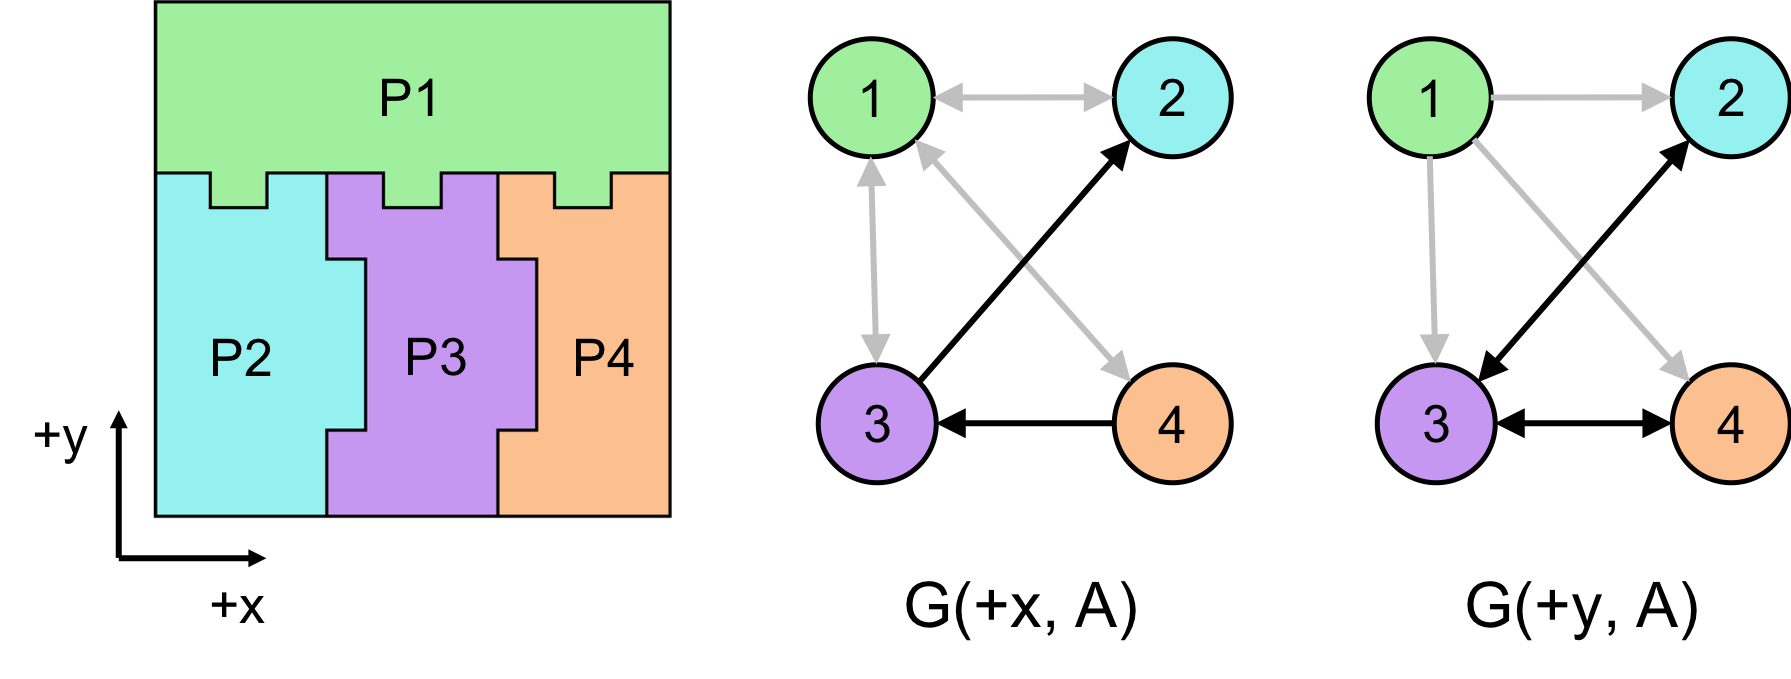
\includegraphics[width=8.45cm]{images/non-recursive_interlocking.png}
	\vspace*{-2.5mm}
	\caption{A non-recursive interlocking 2D puzzle $A$. The dark black edges in $G(+x, A)$ do not form a cycle, which means $[P_2, P_3, P_4]$ is not interlocking. Therefore, the assembly $A$ is not recursive interlocking.
	}
	\vspace*{-4.5mm}
	\label{fig:non-recursive interlocking}
\end{figure}

An non-recursive interlocking example is given in Fig.\ref{fig:non-recursive interlocking}. Given a general voxelized shape $S$, the solution number of recursive interlocking accounts for a small proportion of general interlocking and the proportion will dramatically drop when the number of parts increase. It can be explained in two aspects.

\vspace*{2mm}
\noindent
{\bf Cycle in DBGs: } The recursive interlocking usually has cycles with less than 4 vertices for any DBGs. The local interlocking group $[P_{i}, P_{i+1}, P_{i+2}]$ constrain the cycle size.

\vspace*{2mm}
\noindent
{\bf Disassembling sequence: } The recursive interlocking only have two (the order of last two pieces can be swapped) possible disassembling sequence. The general interlocking in Fig.\ref{fig:non-recursive interlocking} has four disassembling sequences:
\begin{equation*}
	(1, 2, 3, 4), (1, 2, 4, 3), (1, 4, 2, 3), (1, 4, 3, 2)
\end{equation*}

\subsection{Failure Cases and Modification}
\label{subsec: failurecases}
Lastly, inspired by our DBG-based representation, we find that a parts-graph with a cut point cannot be interlocking, no matter what kinds of joints are planned; see Figure~\ref{fig:Result_Furniture_Chair}(left) for an example.
This observation allows us to modify a given input to make it possible to be interlocking by adding a minimal number of new parts in the parts-graph in oder to remove the cut point; see Figure~\ref{fig:Result_Furniture_Chair}(right) for an example.

\begin{figure}[!t]
	\centering
	%\vspace*{-3.5mm}
	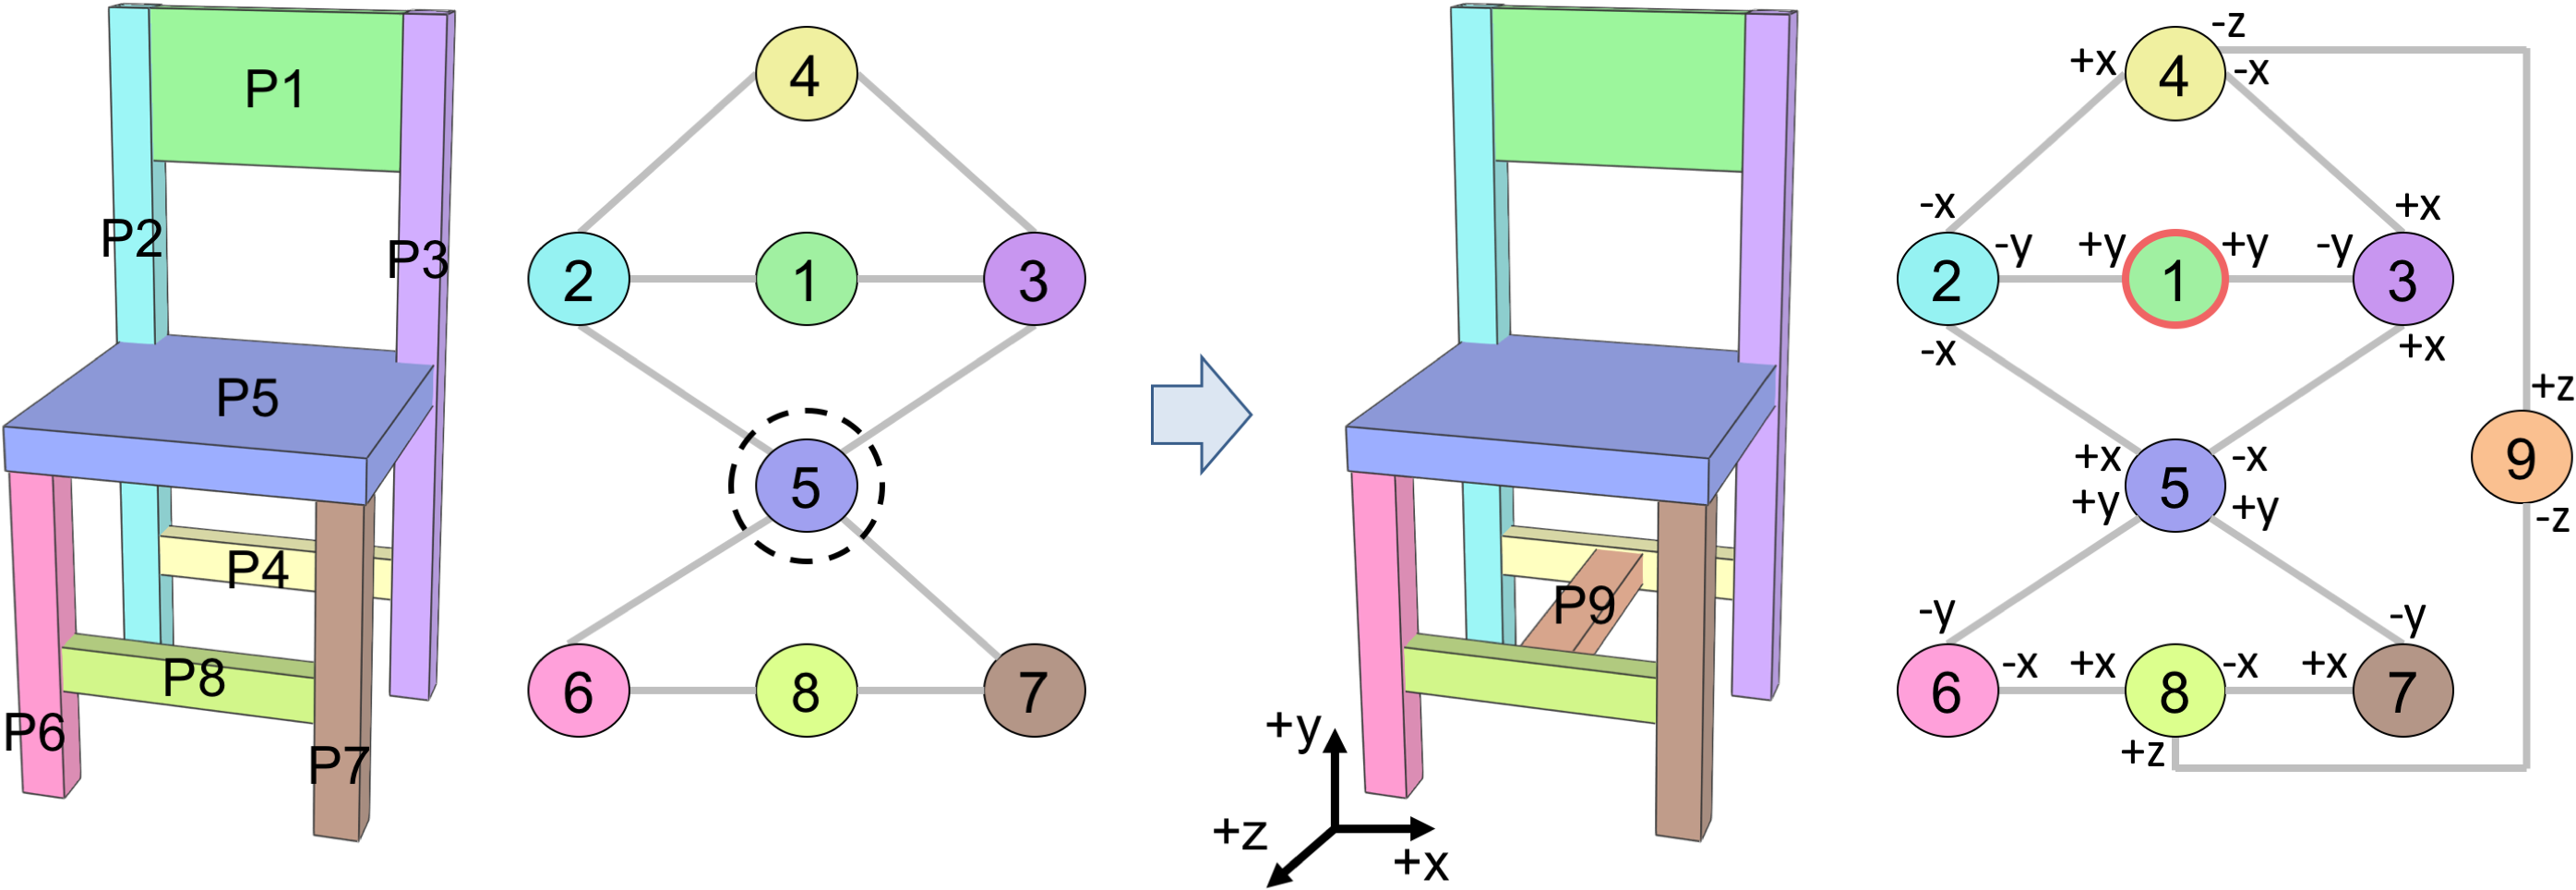
\includegraphics[width=8.45cm]{images/Result_Furniture_Chair.png}
	\vspace*{-2.5mm}
	\caption{
		Left: a {\textsc Chair} and its parts-graph, where a cut point (i.e., $P_5$) exists.
		Right: after adding a new part (i.e., $P_9$), our approach can generate an interlocking joint configuration, where the axial removal direction allowed by each joint is shown in the corresponding edge in the parts-graph. 
	}
	\vspace*{-4.5mm}
	\label{fig:Result_Furniture_Chair}
\end{figure}